% Generated by experiments/exp2_thesis/make_assets.py -- do not edit by hand.
\begin{figure}[tbp]
  \centering
  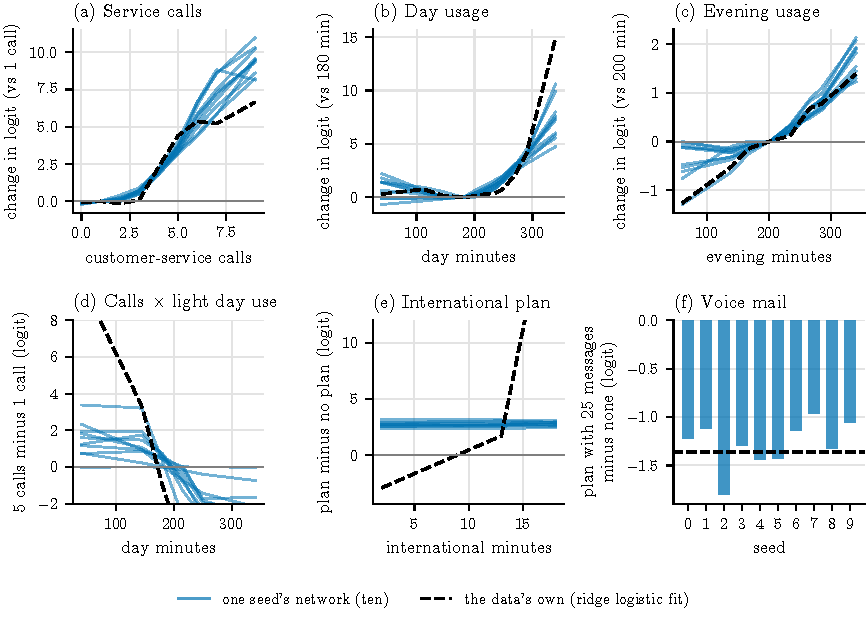
\includegraphics[width=\textwidth]{figures/exp2/exp2-churn-shapes}
  \caption{Churn: each signal's shape as realised in the ten networks (one line per seed), against the data's own shape (dashed). Each curve is the network's component for that signal, projected on the training rows, as a change in the churn score (logit); other inputs are at their training mean. (a)--(c) and (f) agree closely across seeds. (d) The seeds share one shape for calls $\times$ light day use, weaker than the data's. (e) Every network treats the international plan as a flat offset, while the data's effect rises steeply among plan holders with more than 13 international minutes (the interaction in Table~\ref{tab:exp2-churn-blindspot}); the data's curve is a ridge fit and extrapolates where customers are few.}
  \label{fig:exp2-churn-shapes}
\end{figure}
